\section{Program representations and querying mechanisms} %OK

Programs can be represented in several ways. These representations can then be queried to detect all kinds of information, such as control- and data-flow properties. In this section, three program representation approaches are presented, together some means to query those representations.

\subsection{Exploring and Enforcing Security Guarantees via Program Dependence Graphs}
% PidginQL (Queries PDG) JOANA ook PDG

\subsection{GATEKEEPER: Mostly Static Enforcement of Security and Reliability Policies for JavaScript Code}
% Datalog (Gatekeeper)
% Statisch analyse deel van PQL is ook in datalog

\subsection{Parametric regular path queries}
% Mijn algoritme (+ eclipse plugin bespreken)

\section{Expressing policies using a domain-specific language} %OK

This section describes three internal domain-specific languages (\textit{DSL}s). We present one DSL written in Java, a statically typed language, and two DSLs written in dynamically typed languages, namely Ruby and JavaScript.

\subsection{Fluent Interfaces to a Java-Based Internal Domain-Specific Languages for Graph Generation and Analysis}
% Java paper voor graphs
Many complex systems problems manifest themselves as networks. Reasoning about these networks can be hard to do manually and asks for complex algorithms to perform sometimes even simple calculations. Hawick\cite{FluentInterfacesJava} pleads for the use of some sort of abstraction to perform graph generation and analysis, more specifically the use of an internal domain-specific language. He presents a DSL built using fluent interface techniques and the statically typed Java programming language. Common data structures and repetitive computations often offer an opportunity to abstract over them, as is the case for models based on networks and graphs.

The goal of this graph DSL is to be able to compare individual network sets to detect chatacteristic signature properties. The approach is powerful because a major set of data structures and operations on graphs can be abstracted into a library framework, which can then be used by domain experts. 

The first step in setting up the DSL is to set up the common data structures. For the graph DSL, there are three: \texttt{Node}s, \texttt{Arc}s and of course the \texttt{Graph}s themselves. The fields of these data structures are divided into several categories, as depicted in figure \ref{fig:DataStructuresJava}. Structural fields hold the main graph structure, whereas auxiliaries just exist to facilitate computations. Convenience fields contain information that might come in handy, but isn't necessarily used for computations. Finally, decorative fields just are there to have some means of presenting the data in a clear, distinguishable way.

\begin{figure}[!ht]
  	\centering
    	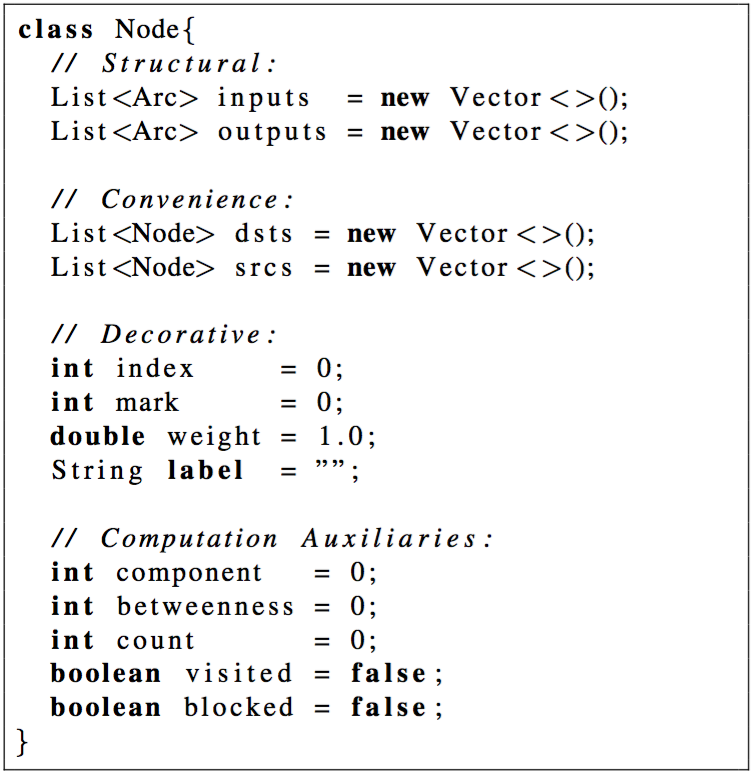
\includegraphics[width=0.5\textwidth]{images/DataStructuresJava} 
    	\caption{The 'Node' data structure}
    \label{fig:DataStructuresJava}
\end{figure}

Since we now have all information to perform most of the complex computations, the fluent interface can be set up. The approach used here implements the (Java) method chaining technique. This enables the cascading of methods by making each method in the fluent interface return the reference to itself, namely the \textit{this} reference. 

Most internal DSL's can be used as a standalone language, as seen in figure \ref{fig:MethodChainingJava}, but the paper also gives some examples in which the DSL is used inside the host language, such as the repetitive removal of the most stressed node in the network to investigate network robustness.

\begin{figure}[!ht]
  	\centering
    	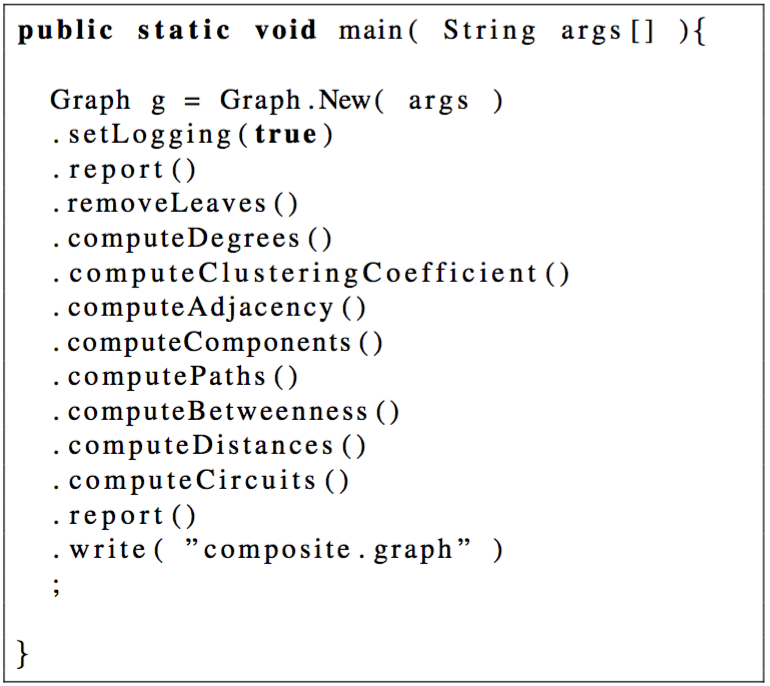
\includegraphics[width=0.5\textwidth]{images/MethodChainingJava} 
    	\caption{Example use of the internal DSL}
    \label{fig:MethodChainingJava}
\end{figure}

\subsection{A Little Language for Surveys: Constructing an Internal DSL in Ruby}
% Ruby paper
A Little Language for Surveys \cite{RubyDSL} explores the use of the Ruby programming language to implement an internal domain-specific language. It checks how well the flexible and dynamic nature of the language accomodates for the implementation of a DSL for specifying and executing surveys. Two key features of the Ruby programming languages are exploited because they especially support defining internal DSLs : The flexibility of the syntax\cite{RubyFlexibleSupport} and the support for blocks\cite{RubyBlockSupport}. Figure \ref{fig:RubySyntax} shows how function calls are easily readable, since the braces surrounding the arguments can be omitted and the arguments list can consist of a variable number of arguments (The latter is also supported in JavaScript\cite{Ecma6}). It also shows how entire blocks can be attached to method calls. These blocks are passed unevaluated to the called method, enabling \textit{deferred evaluation}.

\begin{figure}[!ht]
  	\centering
    	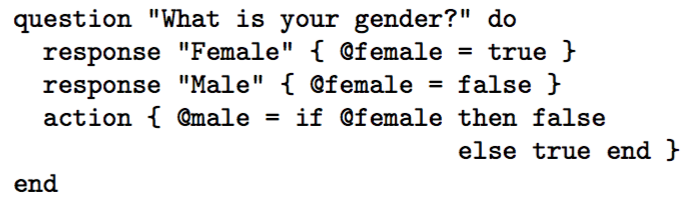
\includegraphics[width=0.75\textwidth]{images/RubySyntax} 
    	\caption{Ruby method call syntax}
    \label{fig:RubySyntax}
\end{figure}

A handy feature in programming languages is reflexive metaprogramming. The survey DSL makes use of the following Ruby reflexive metaprogramming facilities:

\begin{description}[align=left]

\item [obj.instance\_eval(str)] takes a string \texttt{str} and executes it as Ruby code in the context of \texttt{obj}. This method allows internal DSL code from a string or file to be executed by the Ruby interpreter.

\item [mod.class\_eval(str)] takes a string \texttt{str} and executes it as Ruby code in the context of module \texttt{mod}. This enables new methods and classes to be declared dynamically in the running program.
\item [obj.method\_missing(sym, *args)] is invoked when there is an attempt to call an undefined method with the name \texttt{sym} and argument list \texttt{args} on the object \texttt{obj}. This enables the object to take appropriate remedial action.
\item [obj.send(sym, *args)] calls method \texttt{sym} on object \texttt{obj} with argument list \texttt{args}. In Ruby terminology, this sends a message to the object.
\end{description}

The design of the survey language is fairly simple. A survey consists of a title, some questions, some responses and finally a result. Each of these actions have a corresponding method in the DSL.

The developers of the survey language chose to split up the parsing and interpretation logic, following the \textit{two-pass architecture}.
% First pass
The first-pass layer parses the file (which is read using \texttt{instance\_eval}) and generates an abstract syntax tree. These parser classes are structured according to the \textit{Object Scoping} pattern\cite{DSLFowler}, using an approach called \textit{sandboxing}. This architecture is depicted in figure \ref{fig:RubyDSLArchitecture}. The \texttt{SurveyBuilder} class evaluates the statements it reads from the input file using it's superclass' methods. This evaluation parses the input file and builds the AST, which is stored in the superclass as well. In this way, the object scoping pattern is applied: All calls are directed to a single object (the superclass), and global namespace cluttering is avoided. When creating the AST nodes, all blocks that were passed to the method calls inside the top-level call are stored in the AST nodes, instead of being evaluated directly. These blocks will only be evaluated in the second-pass phase (hence \textit{deferred evaluation}). This is illustrated in figure \ref{fig:RubySyntax}, where the block passed to \texttt{question} is evaluated in the first-pass layer, and the blocks passed to \texttt{response} and \texttt{action} are stored in the AST, ready to be evaluated in the second-pass layer.
Note that sandboxing occurs by calling \texttt{instance\_eval} inside the \texttt{SurveyBuilder} object. In this way, harm can only be done \textit{inside} this object. 

\begin{figure}[!ht]
  	\centering
    	\includegraphics[width=0.2\textwidth]{images/RubyDSLArchitecture} 
    	\caption{The survey language DSL architecture}
    \label{fig:RubyDSLArchitecture}
\end{figure}

% Second pass
The actual interpretation of the created AST happens in the second-pass layer. This is a design decision which allows for different interpretation layers to be plugged in/swapped on-the-fly. However, for the survey language a simple \textit{visitor} pattern implementation suffices to process the AST. Every AST node must provide an \texttt{accept} method which takes a \texttt{SurveyVisitor} as an argument. This is the only condition that has to be met by the interpretation layer. In this concrete example, there could be a \texttt{SurveyConsoleVisitor} and a \texttt{SurveyGUIVisitor} class, each representing the survey in their own specific way.



\subsection{Dagoba: an in-memory graph database}
% 500 lines or less

\section{Conclusion}